%----------------------------------------------------------------------------------------
%	VARIOUS REQUIRED PACKAGES AND CONFIGURATIONS
%----------------------------------------------------------------------------------------

\usepackage[top=3cm,bottom=3cm,left=3cm,right=3cm,headsep=10pt,a4paper]{geometry} % Page margins
 
\usepackage{graphicx} 
\usepackage[english]{babel}
%\usepackage{enumitem} % Customize lists
% \setlist{nolistsep} % Reduce spacing between bullet points and numbered lists
% 
% \usepackage{booktabs} % Required for nicer horizontal rules in tables
% 
% \usepackage{marvosym}
% 
\usepackage{xcolor} % Required for specifying colors by name
\definecolor{black}{rgb}{0.1,0.1,0.1} % Define the orange color used for
\definecolor{grey}{rgb}{0.7,0.7,0.9} % Define the orange color used for
\definecolor{darkgrey}{rgb}{0.1,0.1,0.1} % Define the orange color used for
\definecolor{ocre}{RGB}{243,102,25} % Define the orange color used for highlighting throughout the book
\definecolor{green}{RGB}{25,243,102} % Define the orange color used for
% highlighting throughout the book \definecolor{aureolin}{rgb}{0.99, 0.93, 0.0} % Define the yellow color used for
% 
% \definecolor{airforceblue}{rgb}{0.36, 0.54, 0.66}% Define the blue color used for
% 
% 


\parskip 1.5ex % paragraph spacing

 
% %----------------------------------------------------------------------------------------
% %	THEOREM STYLES
% %----------------------------------------------------------------------------------------
% 
% \usepackage{amsmath,amsfonts,amssymb,amsthm} % For math equations, theorems, symbols, etc
% 
% \newcommand{\intoo}[2]{\mathopen{]}#1\,;#2\mathclose{[}}
% \newcommand{\ud}{\mathop{\mathrm{{}d}}\mathopen{}}
% \newcommand{\intff}[2]{\mathopen{[}#1\,;#2\mathclose{]}}
% \newtheorem{notation}{Notation}[chapter]
% 
% % Boxed/framed environments
% \newtheoremstyle{ocrenumbox}% % Theorem style name
% {0pt}% Space above
% {0pt}% Space below
% {\normalfont}% % Body font
% {}% Indent amount
% {\small\bf\sffamily\color{ocre}}% % Theorem head font
% {\;}% Punctuation after theorem head
% {0.25em}% Space after theorem head
% {\small\sffamily\color{ocre}\thmname{#1}\nobreakspace\thmnumber{\@ifnotempty{#1}{}\@upn{#2}}% Theorem text (e.g. Theorem 2.1)
% \thmnote{\nobreakspace\the\thm@notefont\sffamily\bfseries\color{black}---\nobreakspace#3.}} % Optional theorem note
% \renewcommand{\qedsymbol}{$\blacksquare$}% Optional qed square
% 
% \newtheoremstyle{blacknumex}% Theorem style name
% {5pt}% Space above
% {5pt}% Space below
% {\normalfont}% Body font
% {} % Indent amount
% {\small\bf\sffamily}% Theorem head font
% {\;}% Punctuation after theorem head
% {0.25em}% Space after theorem head
% {\small\sffamily{\tiny\ensuremath{\blacksquare}}\nobreakspace\thmname{#1}\nobreakspace\thmnumber{\@ifnotempty{#1}{}\@upn{#2}}% Theorem text (e.g. Theorem 2.1)
% \thmnote{\nobreakspace\the\thm@notefont\sffamily\bfseries---\nobreakspace#3.}}% Optional theorem note
% 
% \newtheoremstyle{blacknumbox} % Theorem style name
% {0pt}% Space above
% {0pt}% Space below
% {\normalfont}% Body font
% {}% Indent amount
% {\small\bf\sffamily}% Theorem head font
% {\;}% Punctuation after theorem head
% {0.25em}% Space after theorem head
% {\small\sffamily\thmname{#1}\nobreakspace\thmnumber{\@ifnotempty{#1}{}\@upn{#2}}% Theorem text (e.g. Theorem 2.1)
% \thmnote{\nobreakspace\the\thm@notefont\sffamily\bfseries---\nobreakspace#3.}}% Optional theorem note
% 
% % Non-boxed/non-framed environments
% \newtheoremstyle{ocrenum}% % Theorem style name
% {5pt}% Space above
% {5pt}% Space below
% {\normalfont}% % Body font
% {}% Indent amount
% {\small\bf\sffamily\color{ocre}}% % Theorem head font
% {\;}% Punctuation after theorem head
% {0.25em}% Space after theorem head
% {\small\sffamily\color{ocre}\thmname{#1}\nobreakspace\thmnumber{\@ifnotempty{#1}{}\@upn{#2}}% Theorem text (e.g. Theorem 2.1)
% \thmnote{\nobreakspace\the\thm@notefont\sffamily\bfseries\color{black}---\nobreakspace#3.}} % Optional theorem note
% \renewcommand{\qedsymbol}{$\blacksquare$}% Optional qed square
% \makeatother
% 
% % Defines the theorem text style for each type of theorem to one of the three styles above
% \newcounter{dummy} 
% \numberwithin{dummy}{section}
% \theoremstyle{ocrenumbox}
% \newtheorem{theoremeT}[dummy]{Theorem}
% \newtheorem{problem}{Problem}[chapter]
% \newtheorem{exerciseT}{Exercise}[chapter]
% \newtheorem{designT}{Design philosophy}[chapter]
% \theoremstyle{blacknumbox}
% \newtheorem{infoT}{Note}[chapter] % icon: \Info
% \newtheorem{warningT}{Warning}[chapter] % icon: \danger
% \newtheorem{exampleT}{Example}[chapter]
% \theoremstyle{blacknumbox}
% \newtheorem{vocabulary}{Vocabulary}[chapter]
% \newtheorem{definitionT}{Definition}[section]
% \newtheorem{corollaryT}[dummy]{Corollary}
% \theoremstyle{ocrenum}
% \newtheorem{proposition}[dummy]{Proposition}
% 
% %----------------------------------------------------------------------------------------
% %	DEFINITION OF COLORED BOXES
% %----------------------------------------------------------------------------------------
% 
% \RequirePackage[framemethod=default]{mdframed} % Required for creating the theorem, definition, exercise and corollary boxes
% 
% % Theorem box
% \newmdenv[skipabove=7pt,
% skipbelow=7pt,
% backgroundcolor=black!5,
% linecolor=ocre,
% innerleftmargin=5pt,
% innerrightmargin=5pt,
% innertopmargin=5pt,
% leftmargin=0cm,
% rightmargin=0cm,
% innerbottommargin=5pt]{tBox}
% 
% % Exercise box	  
% \newmdenv[skipabove=7pt,
% skipbelow=7pt,
% rightline=false,
% leftline=true,
% topline=false,
% bottomline=false,
% backgroundcolor=ocre!10,
% linecolor=ocre,
% innerleftmargin=5pt,
% innerrightmargin=5pt,
% innertopmargin=5pt,
% innerbottommargin=5pt,
% leftmargin=0cm,
% rightmargin=0cm,
% linewidth=4pt]{eBox}	
% 
% % Definition box
% \newmdenv[skipabove=7pt,
% skipbelow=7pt,
% rightline=false,
% leftline=true,
% topline=false,
% bottomline=false,
% linecolor=ocre,
% innerleftmargin=5pt,
% innerrightmargin=5pt,
% innertopmargin=0pt,
% leftmargin=0cm,
% rightmargin=0cm,
% linewidth=4pt,
% innerbottommargin=0pt]{dBox}
% 
% % Corollary box
% \newmdenv[skipabove=7pt,
% skipbelow=7pt,
% rightline=false,
% leftline=true,
% topline=false,
% bottomline=false,
% linecolor=gray,
% backgroundcolor=black!5,
% innerleftmargin=5pt,
% innerrightmargin=5pt,
% innertopmargin=5pt,
% leftmargin=0cm,
% rightmargin=0cm,
% linewidth=4pt,
% innerbottommargin=5pt]{cBox}
% 
% % Corollary style
% \mdfdefinestyle{cBoxStyle}{%
% skipabove=7pt,
% skipbelow=7pt,
% rightline=false,
% leftline=true,
% topline=false,
% bottomline=false,
% linecolor=gray,
% backgroundcolor=black!5,
% innerleftmargin=5pt,
% innerrightmargin=5pt,
% innertopmargin=5pt,
% leftmargin=0cm,
% rightmargin=0cm,
% linewidth=4pt,
% innerbottommargin=5pt
% }
% 
% % Warning box
% \newmdenv[skipabove=7pt,
% skipbelow=7pt,
% rightline=false,
% leftline=true,
% topline=false,
% bottomline=false,
% linecolor=aureolin, 
% backgroundcolor=aureolin!20,
% innerleftmargin=5pt,
% innerrightmargin=5pt,
% innertopmargin=5pt,
% innerbottommargin=5pt,
% leftmargin=0cm,
% rightmargin=0cm,
% linewidth=4pt,
% innerbottommargin=0pt]{wBox}
% 
% % Info box
% \newmdenv[skipabove=7pt,
% skipbelow=7pt,
% rightline=false,
% leftline=true,
% topline=false,
% bottomline=false,
% linecolor=airforceblue, 
% backgroundcolor=airforceblue!20,
% innerleftmargin=5pt,
% innerrightmargin=5pt,
% innertopmargin=5pt,
% innerbottommargin=5pt,
% leftmargin=0cm,
% rightmargin=0cm,
% linewidth=4pt,
% innerbottommargin=0pt]{iBox}
% 
% % Creates an environment for each type of theorem and assigns it a theorem text style from the "Theorem Styles" section above and a colored box from above
% \newenvironment{theorem}{\begin{tBox}\begin{theoremeT}}{\end{theoremeT}\end{tBox}}
% \newenvironment{exercise}{\begin{eBox}\begin{exerciseT}}{\hfill{\color{ocre}\tiny\ensuremath{\blacksquare}}\end{exerciseT}\end{eBox}}	
% \newenvironment{design}{\begin{eBox}\begin{designT}}{\end{designT}\end{eBox}}
% \newenvironment{definition}{\begin{dBox}\begin{definitionT}}{\end{definitionT}\end{dBox}}	
% \newenvironment{example}{\begin{exampleT}}{\hfill{\tiny\ensuremath{\blacksquare}}\end{exampleT}}		
% \newenvironment{corollary}{\begin{cBox}\begin{corollaryT}}{\end{corollaryT}\end{cBox}}	
% \newenvironment{warning}{\begin{wBox}\begin{warningT}}{\end{warningT}\end{wBox}}
% \newenvironment{info}{\begin{iBox}\begin{infoT}}{\end{infoT}\end{iBox}}
% 
% %----------------------------------------------------------------------------------------
% %	REMARK ENVIRONMENT
% %----------------------------------------------------------------------------------------
\usepackage{tikz} 


\newenvironment{remark}{\par\vspace{10pt}\small % Vertical white space above the remark and smaller font size
 \begin{list}{}{
 \leftmargin=35pt % Indentation on the left
 \rightmargin=25pt}\item\ignorespaces % Indentation on the right
 \makebox[-2.5pt]{\begin{tikzpicture}[overlay]
 \node[draw=green!60,line
 width=1pt,circle,fill=green!25,font=\sffamily\bfseries,inner sep=2pt,outer
 sep=0pt] at (-15pt,0pt){\textcolor{black}{R}};\end{tikzpicture}} % Orange R in
 % a circle
 \advance\baselineskip -1pt}{\end{list}\vskip5pt} % Tighter line spacing and white space after remark


\newenvironment{definition}{\par\vspace{10pt}\small 
 \begin{list}{}{
 \leftmargin=35pt % Indentation on the left
 \rightmargin=25pt}\item\ignorespaces % Indentation on the right
 \makebox[-2.5pt]{
\begin{tikzpicture}[overlay]
 \node[draw=ocre!60,line
 width=1pt,circle,fill=ocre!25,font=\sffamily\bfseries,inner sep=2pt,outer sep=0pt] at (-15pt,0pt){\textcolor{ocre}{D}};\end{tikzpicture}} % Orange R in a circle
 \advance\baselineskip -1pt}{\end{list}\vskip5pt} % Tighter line spacing and white space after remark
 
% %----------------------------------------------------------------------------------------
% %	SECTION NUMBERING IN THE MARGIN
% %----------------------------------------------------------------------------------------
% 
% \makeatletter
% \renewcommand{\@seccntformat}[1]{\llap{\textcolor{ocre}{\csname the#1\endcsname}\hspace{1em}}}                    
% \renewcommand{\section}{\@startsection{section}{1}{\z@}
% {-4ex \@plus -1ex \@minus -.4ex}
% {1ex \@plus.2ex }
% {\normalfont\large\sffamily\bfseries}}
% \renewcommand{\subsection}{\@startsection {subsection}{2}{\z@}
% {-3ex \@plus -0.1ex \@minus -.4ex}
% {0.5ex \@plus.2ex }
% {\normalfont\sffamily\bfseries}}
% \renewcommand{\subsubsection}{\@startsection {subsubsection}{3}{\z@}
% {-2ex \@plus -0.1ex \@minus -.2ex}
% {.2ex \@plus.2ex }
% {\normalfont\small\sffamily\bfseries}}                        
% \renewcommand\paragraph{\@startsection{paragraph}{4}{\z@}
% {-2ex \@plus-.2ex \@minus .2ex}
% {.1ex}
% {\normalfont\small\sffamily\bfseries}}
% 
 
\usepackage{hyperref}
\hypersetup{hidelinks,backref=true,pagebackref=true,hyperindex=true,colorlinks=false,breaklinks=true,urlcolor= ocre,bookmarks=true,bookmarksopen=false,pdftitle={Title},pdfauthor={Author}}

\hypersetup{
  pdftitle={Peano Cookbook},
  pdfauthor={Tobias Weinzierl},
  pdfsubject={Peano Cookbook}
}


\newcommand{\Peano}{Peano~4}
\newcommand{\ExaHyPE}{ExaHyPE~2}


\usepackage{listings}


\lstdefinelanguage{cCCode}[]{C}{
   backgroundcolor=\color{grey},
 %  basicstyle=\tiny,
 %  basicstyle=\Small,
   basicstyle=\footnotesize,
   stringstyle=\color{red},
   keywordstyle=\color{blue},
   commentstyle=\color{darkgrey}\slshape,
   morekeywords={linestyle,linetype,linewidth,linecolor,pointtype,nohidden3d,hidden3d,palette,lt,lw,lc,pt,ps,fd,fill,fs,ls},
   framexleftmargin=1mm, framextopmargin=1mm, frame=shadowbox,
   rulesepcolor=\color{darkgrey}
 }

 
 
     
\lstnewenvironment{code}[1][]{
\lstset{
 language=cCCode,#1,
 upquote=true,
 columns=fullflexible,
 literate={*}{{\char42}}1
          {-}{{\char45}}1
}}{}
     
     
